\section{Introducción a LabMan}

Es este apartado se realiza una breve introducción a \acrfull{labman}, el \acrlong{dms} del grupo de investigación MoreLab, así como de las tecnologías que lo conforman. Este contexto facilitará la comprensión de los próximos capítulos, además de describir los fundamentos clave para desarrollo de este proyecto.

\begin{figure}[!htp]
	\centering
	
\includegraphics[scale=0.15]{fig/morelab-logo}
	\caption{Logotipo de MORELab}
\end{figure}

Gestionar la información no siempre es una tarea trivial y más aún cuando hay que tratar con los datos que componen varias entidades como pueden ser los proyectos, investigadores, publicaciones, eventos, etc. dentro del ámbito de la investigación. La mayoría de los grupos de investigación utilizan sistemas de gestión de contenido tales como Joomla!\cite{joomla}, WordPress\cite{wordpress} o Drupal\cite{drupal} para exponer sus datos. Sin embargo, para extraer la información de estos \acrshortpl{cms} se requieren herramientas externas para llevar a cabo técnicas de análisis de datos. 
Para hacer uso de estas herramientas normalmente hace falta generar documentos adicionales, tales como \acrshort{csv}, hojas de cálculo, ficheros de texto, generado información redundante, que provoca dificultades a la hora de actualizar los datos y la calidad de los mismos. Esta situación empeora cuando además se disponen de distintas fuentes para la obtención de información, como pueden ser las paginas web personales de los investigadores en los que se muestran sus logros a lo largo de su carrera, la información financiera gestionada por su propio departamento, etc.

\begin{figure}[!htp]
	\centering
	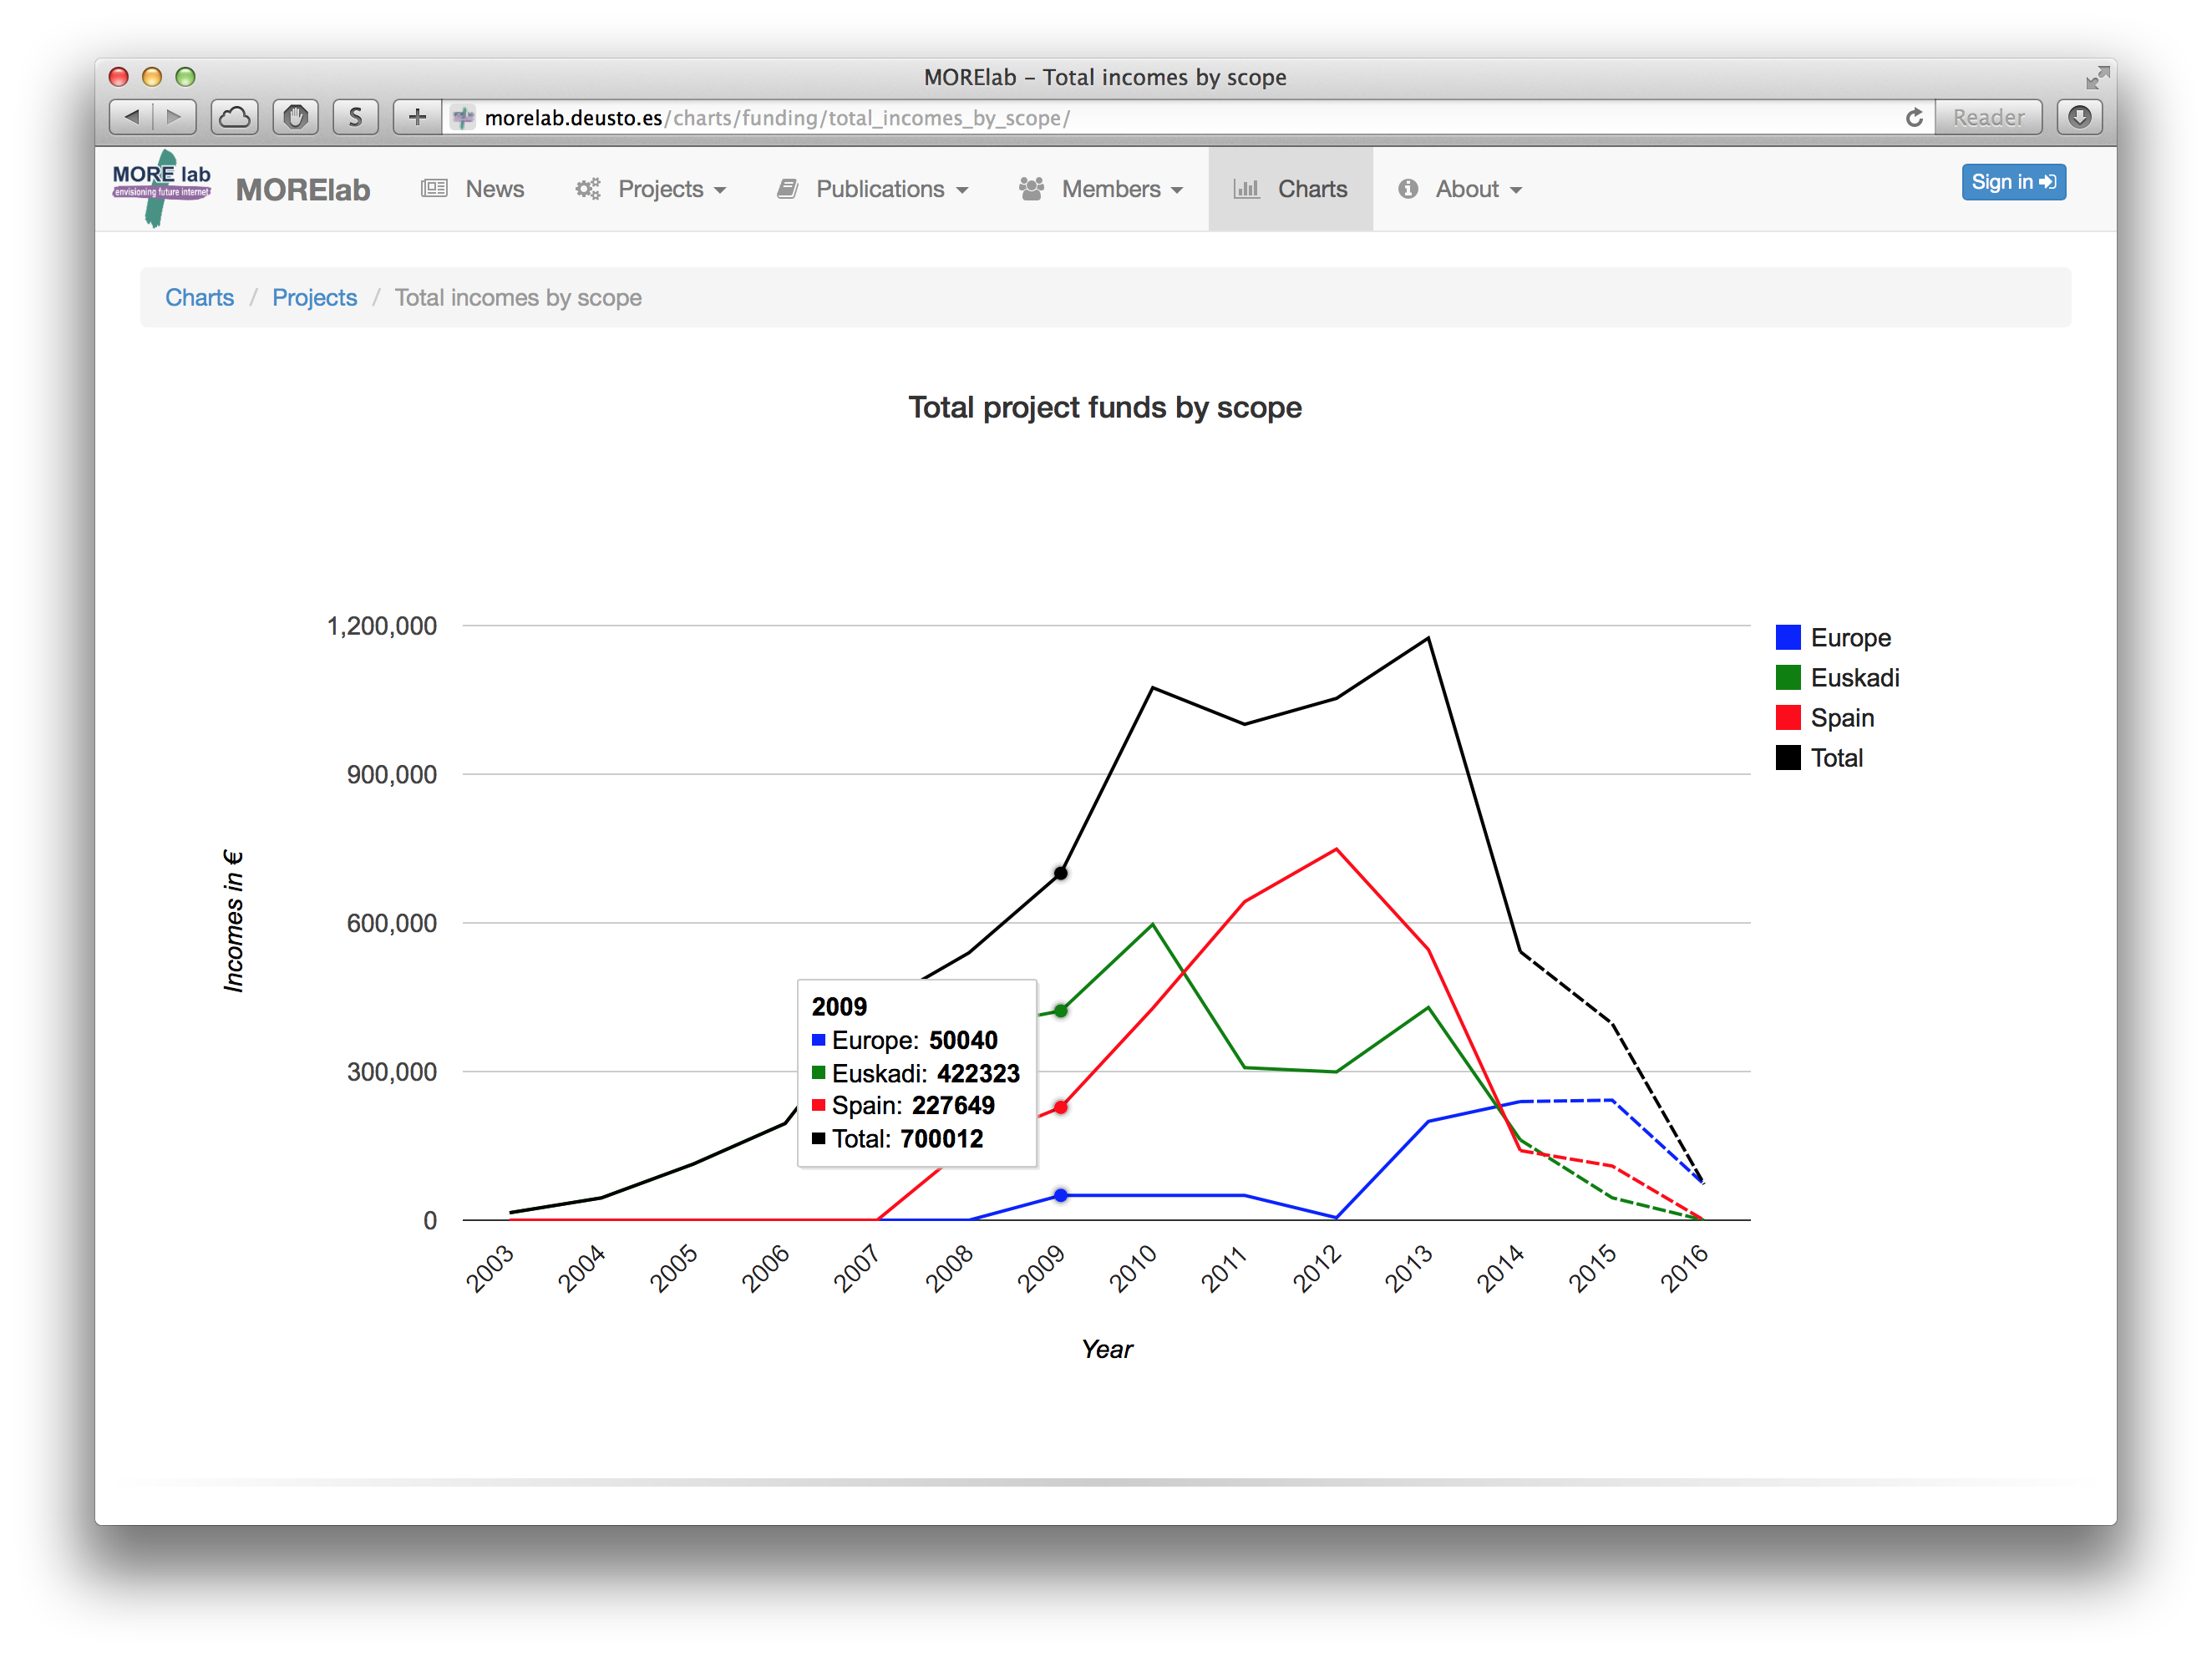
\includegraphics[scale=0.21]{fig/labman-chart}
	\caption{\acrshort{labman}: Gráfico generado por tripletas \acrshort{rdf}}\label{fig:labmanchart}
\end{figure}

Del esfuerzo para gestionar la información grupo de investigación de MoreLab nace \acrshort{labman}, una aplicación desarrollada en Python\cite{Python} por medio del framework para desarrollo web Django\cite{Django} y que sustituye a la antigua solución Joomla! para la publicación de los datos sobre las publicaciones en \acrfull{rdf}\cite{RDF}. Su principal objetivo es gestionar no solo la información relacionada a las publicaciones, sino que va más allá publicando la información relacionada a los proyectos del equipo, sus financiaciones, integrantes de proyecto, noticias de una forma gráfica e intuitiva tal y como se puede ver en la figura \ref{fig:labmanchart}, diferenciadose de otros \acrshortpl{cms} por apostar por la exposición de los datos como \acrlong{lod}\cite{linkeddata}, disponible por todos sin restricción de derechos de \textit{copyrights} o patentes. Si es verdad que existen extensiones para que los \acrshort{cms} puedan publicar los datos almacenados en estos sistemas como \acrshortpl{rdf}, no permiten acceder a estos mediante un punto de salida \acrshort{sparql}, por lo que no se pueden realizar consultas complejas a entidades externas ni aprovechar las ventajas que se producen por publicarlos siguiendo las prácticas de \acrshort{ld}.\cite{pena_visual_2014}